% !TEX root = main.tex
% !TEX encoding = UTF-8
% !TEX program = pdflatex

\section{Network Models}
    In this section we describe how we developed the algorithms to generate the synthetic networks and than the Facebook network.
    
    To develop this models we decided to use \textbf{Python} because is a easy and very flexible language, in addition there are many libraries and documentation related to our topic.
    We chose to use the library \textit{NetworkX}~\cite{NetworkX} because this library have a very fast learning curve.
    
    We made the assumption that the population are fully mixed, as described in this paper \cite{witten2007simulations}, so the susceptible population have a fixed probability $\beta$ per unit time to get the disease from any infected neighbour. The set of neighbour of a vertex $v \in V$ is denoted with $N_G(v) = \{u_1, u_2, ..., u_i \}$, where $u_k,~k=1,...,i$, is adjacent to a given vertex \verb|v|.
    Than we need to define the fixed probability $\gamma$ per unit time that represent the probability to be recovered/immunised.
    With this parameter we can model the population susceptible, infected and recovered by a system of ordinary differential equation \ref{eq:diffEq} proposed in the paper~\cite{witten2007simulations}:
    
    \begin{equation}\label{eq:diffEq}
      \left\{\begin{matrix}
        \frac{\mathrm{d} s}{\mathrm{d} t} = -\beta si, & 
        \frac{\mathrm{d} i}{\mathrm{d} t} = \beta si - \gamma i,& 
        \frac{\mathrm{d} r}{\mathrm{d} t} = \gamma i
    \end{matrix}\right.
    \end{equation}
    where s,i,r are respective the number of susceptible, infected and recovered person at that moment.
    Where s in not increasing, i is not decreasing and the last equation is redundant since $(d/dt)(s + i + r) = 0$ implies that $s +i +r = N$, with \verb|N| the total number of nodes of graph $|V| \in G$, at all times.
    
    \subsection{Random Network}
        In this section we will describe how we implemented the random network generator.
        
        \begin{lstlisting}[language=Python, frame=single]]
import networkx as nx

# population number
N = 1000

# probability p of any two sites being
    connected
P = 0.001

# create a network with random neighboUr
# numberOfNodes: number of nodes of this
    graph
# neighborProbability: probability to 
    establish a link between two nodes
    
def createRandomNetwork():
    # create a new Graph for our social
        network
    G = nx.Graph(name='RandomNetwork')
    
    # generate N nodes
    for i in range(N):
        G.add_node("node"+str(i), 
            state = sirv.SUSCEPTIBLE,
            dayOfInfection = -1)

    # generate random link
    for source in G:
        for possibleNeighbor in G:
            if(source != possibleNeighbor
                and random() < P):
                
                G.add_edge(source,
                    possibleNeighbor)
    return G
        \end{lstlisting}
        
        At the beginning we defined the number of nodes and the probability that a node have to establish a link with an other node. Then, in the function \verb|createRandomNetwork| we define the nodes and we generate a random number and make a comparison with the threshold, the probability that that node establish a connection, and if the random number is lower than the threshold we add that link to the graph \verb|G|.
        
        Because of the nature of random number, the nodes' degree distribution will follow the Poisson distribution, defined by the Eq.\ref{eq:poisson}.
        \begin{equation}\label{eq:poisson}
          p(k) \approx \frac{\lambda^ke^{-\lambda}}{k!}
        \end{equation}
        The parameter $\lambda = N P$, where $N = |V|$ and \verb|P| is the probability to establish a connection. So we can interact with P to decide the shape of this curve, as showed in Fig.\ref{fig:poissonDistribution}\cite{wiky-Poisson}.
        
        \begin{figure}[t]
            \centering
            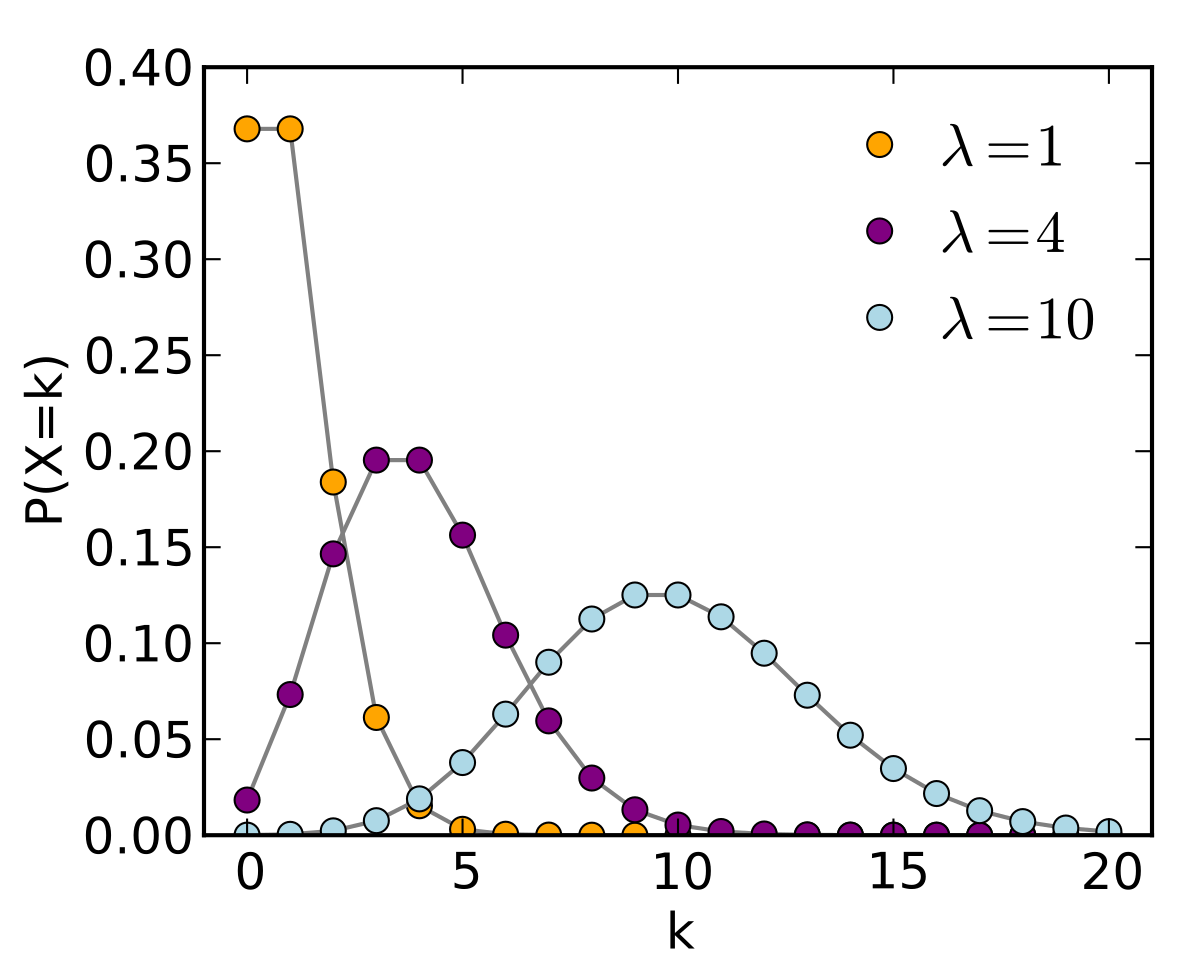
\includegraphics[width=\linewidth]{Figure/poissonDistribution.png}
            \caption{Poisson distribution graph}
            \label{fig:poissonDistribution}
        \end{figure}